\documentclass[11pt]{aghdpl}
% \documentclass[en,11pt]{aghdpl}  % praca w języku angielskim

% Lista wszystkich języków stanowiących języki pozycji bibliograficznych użytych w pracy.
% (Zgodnie z zasadami tworzenia bibliografii każda pozycja powinna zostać utworzona zgodnie z zasadami języka, w którym dana publikacja została napisana.)
\usepackage[english,polish]{babel}

% Użyj polskiego łamania wyrazów (zamiast domyślnego angielskiego).
\usepackage{polski}

\usepackage[utf8]{inputenc}

% dodatkowe pakiety

\usepackage{mathtools}
\usepackage{amsfonts}
\usepackage{amsmath}
\usepackage{amsthm}

% --- < bibliografia > ---

\usepackage[
style=numeric,
sorting=none,
%
% Zastosuj styl wpisu bibliograficznego właściwy językowi publikacji.
language=autobib,
autolang=other,
% Zapisuj datę dostępu do strony WWW w formacie RRRR-MM-DD.
urldate=edtf,
% Nie dodawaj numerów stron, na których występuje cytowanie.
backref=false,
% Podawaj ISBN.
isbn=true,
% Nie podawaj URL-i, o ile nie jest to konieczne.
url=false,
%
% Ustawienia związane z polskimi normami dla bibliografii.
maxbibnames=3,
% Jeżeli używamy BibTeXa:
backend=bibtex
]{biblatex}

\usepackage{csquotes}
% Ponieważ `csquotes` nie posiada polskiego stylu, można skorzystać z mocno zbliżonego stylu chorwackiego.
\DeclareQuoteAlias{croatian}{polish}

\addbibresource{bibliografia.bib}

% Nie wyświetlaj wybranych pól.
%\AtEveryBibitem{\clearfield{note}}


% ------------------------
% --- < listingi > ---

% Użyj czcionki kroju Courier.
\usepackage{courier}

\usepackage{listings}
\lstloadlanguages{TeX}

\lstset{
	literate={ą}{{\k{a}}}1
           {ć}{{\'c}}1
           {ę}{{\k{e}}}1
           {ó}{{\'o}}1
           {ń}{{\'n}}1
           {ł}{{\l{}}}1
           {ś}{{\'s}}1
           {ź}{{\'z}}1
           {ż}{{\.z}}1
           {Ą}{{\k{A}}}1
           {Ć}{{\'C}}1
           {Ę}{{\k{E}}}1
           {Ó}{{\'O}}1
           {Ń}{{\'N}}1
           {Ł}{{\L{}}}1
           {Ś}{{\'S}}1
           {Ź}{{\'Z}}1
           {Ż}{{\.Z}}1,
	basicstyle=\footnotesize\ttfamily,
}

% ------------------------

\AtBeginDocument{
	\renewcommand{\tablename}{Tabela}
	\renewcommand{\figurename}{Rys.}
}

% ------------------------
% --- < tabele > ---

\usepackage{array}
\usepackage{tabularx}
\usepackage{multirow}
\usepackage{booktabs}
\usepackage{makecell}
\usepackage[flushleft]{threeparttable}

% defines the X column to use m (\parbox[c]) instead of p (`parbox[t]`)
\newcolumntype{C}[1]{>{\hsize=#1\hsize\centering\arraybackslash}X}


%---------------------------------------------------------------------------

\author{Łukasz Dudek}
\shortauthor{Ł. Dudek}

%\titlePL{Przygotowanie bardzo długiej i pasjonującej pracy dyplomowej w~systemie~\LaTeX}
%\titleEN{Preparation of a very long and fascinating bachelor or master thesis in \LaTeX}

\titlePL{Dwuczęściowa aplikacja sterowania czasooptymalnego w systemie zbiorników}
\titleEN{A two-part application of time-optimal control in a system of tanks}


\shorttitlePL{Dwuczęściowa aplikacja sterowania czasooptymalnego w systemie zbiorników} % skrócona wersja tytułu jeśli jest bardzo długi
\shorttitleEN{A two-part application of time-optimal control in a system of tanks}

\thesistype{Praca dyplomowa magisterska}
%\thesistype{Master of Science Thesis}

\supervisor{dr hab. inż. Adam Piłat}
%\supervisor{Marcin Szpyrka PhD, DSc}

\degreeprogramme{Automatyka i Robotyka}
%\degreeprogramme{Computer Science}

\date{2017}

\department{Katedra Automatyki i Inżynierii Biomedycznej}
%\department{Department of Applied Computer Science}

\faculty{Wydział Elektrotechniki, Automatyki,\protect\\[-1mm] Informatyki i Inżynierii Biomedycznej}
%\faculty{Faculty of Electrical Engineering, Automatics, Computer Science and Biomedical Engineering}

\acknowledgements{Serdecznie dziękuję mojemu promotorowi, dr hab. inż. Adamowi Piłatowi za cierpliwość.}


\setlength{\cftsecnumwidth}{10mm}

%---------------------------------------------------------------------------
\setcounter{secnumdepth}{4}
\brokenpenalty=10000\relax

\begin{document}

\titlepages

% Ponowne zdefiniowanie stylu `plain`, aby usunąć numer strony z pierwszej strony spisu treści i poszczególnych rozdziałów.
\fancypagestyle{plain}
{
	% Usuń nagłówek i stopkę
	\fancyhf{}
	% Usuń linie.
	\renewcommand{\headrulewidth}{0pt}
	\renewcommand{\footrulewidth}{0pt}
}

\setcounter{tocdepth}{2}
\tableofcontents
\clearpage

\chapter*{Wstęp}
\addcontentsline{toc}{chapter}{Wstęp}

Rozwój techniki komputerowej w ostatnich dziesięcioleciach spowodował szeroki dostęp do metod numerycznych obliczeń problemów analitycznie trudnych bądź niemożliwych do rozwiązywania. W tym momencie skomplikowane algorytmy potrzebujące dużych zasobów sprzętowych można uruchomić na urządzeniach o relatywnie niewielkich rozmiarach.
Skorzystała na tym w oczywisty sposób również automatyka, gdyż metody optymalizacji sterowania w układach nieliniowych stały się możliwe do stosowania w czasie rzeczywistym ze względu na krótki czas obliczeń i niewielkie gabaryty urządzeń wykonujących je.

W obecnych czasach istnieje w automatyce tendencja, aby rozdzielać elementy odpowiedzialne za bezpośrednią komunikację z urządzeniami wykonawczymi od elementów uruchamiających skomplikowane matematycznie algorytmy, aby oba rodzaje można było udoskonalać w wykonywaniu tylko jednej klasy zadań.
Takie podejście zostało również zaprezentowane w niniejszej pracy. Hybrydowa (z łac.: \emph{hybrida}: mieszaniec, krzyżówka) struktura polega na zastosowaniu dwóch poziomów: obliczeniowego i realizującego sterowanie bezpośrednie. 

Niewątpliwą zaletą takiego podejścia jest modułowość: posiadając dobrze określoną specyfikację komunikacji, można bez większego problemu wymienić jeden z elementów składowych takiej aplikacji na inny, szybko tworząc prototypy i testując różne technologie w sposób, który nie zakłóca działania całości aplikacji.

Celem niniejszej pracy jest przygotowanie oprogramowania, będącego w stanie wyliczać i aplikować sterowanie czasooptymalne dla układu trzech zbiorników z wodą. Powinno ono móc również symulować funkcjonowanie tego układu i weryfikować w ten sposób działanie optymalizacji. Dodatkowo powinno umieć podtrzymywać stan docelowy zagadnienia czasooptymalnego przy użyciu regulatora liniowo-kwadratowego.

Pierwszy rozdział niniejszej pracy zawiera opis praw i zjawisk fizycznych, które użyto do wyznaczenia modelu matematycznego rozważanego układu zbiorników. Podano tam również inżynierskie uproszczenia skutkujące prostą strukturą tegoż modelu oraz sam model wraz z jego ograniczeniami.

W drugim rozdziale przytoczono matematyczne podstawy optymalizacji dynamicznej służące do wyznaczenia dwóch rodzajów sterowań optymalnych potrzebnych w niniejszej pracy: czasooptymalnego i liniowo-kwadratowego. Opisano też analityczne i numeryczne metody rozwiązywania pierwszego z tych zagadnień.

Trzeci rozdział jest poświęcony architekturze oprogramowania realizującego cele pracy. Przestawiono tam konkretne zadania dwóch elementów aplikacji o hybrydowej strukturze oraz opisano komunikację między nimi z wyszczególnieniem parametrów wysyłanych przez obie strony.

Techniczny opis zagadnień związanych z oprogramowaniem znajduje się w rozdziale czwartym. Zawiera on opisy użytego oprogramowania, w szczególności tego wykorzystywanego do rozwiązywania zadań optymalizacji dynamicznej.

W ostatnim rozdziale zawarto podsumowanie wszystkich przeprowadzonych badań symulacyjnych. Przedstawiono użyty algorytm optymalizacyjny oraz omówiono jego wyniki. Pokazano sposób na weryfikację otrzymanego rozwiązania na obu poziomach aplikacji i zawarto wnioski z niej płynące.
\chapter{Matematyczny opis zagadnienia}
\label{cha:model}

Rozważany układ składa się z trzech zbiorników połączonych szeregowo, czy też kaskadowo. W związku z tym płyn, którym jest napełniony pierwszy zbiornik - woda - przepływa przez otwór o zadanym oporze wypływu do drugiego zbiornika. Stamtąd znowu wypływa do przez otwór o zadanym oporze do trzeciego zbiornika, skąd przez kolejny taki otwór wypływa do zewnętrznego naczynia. Stamtąd woda jest pompowana z powrotem do pierwszego zbiornika. Całość układu jest przedstawiona schematycznie na rys. \ref{fig:zbiorniki}.


\begin{figure}[ht]
	\centering
	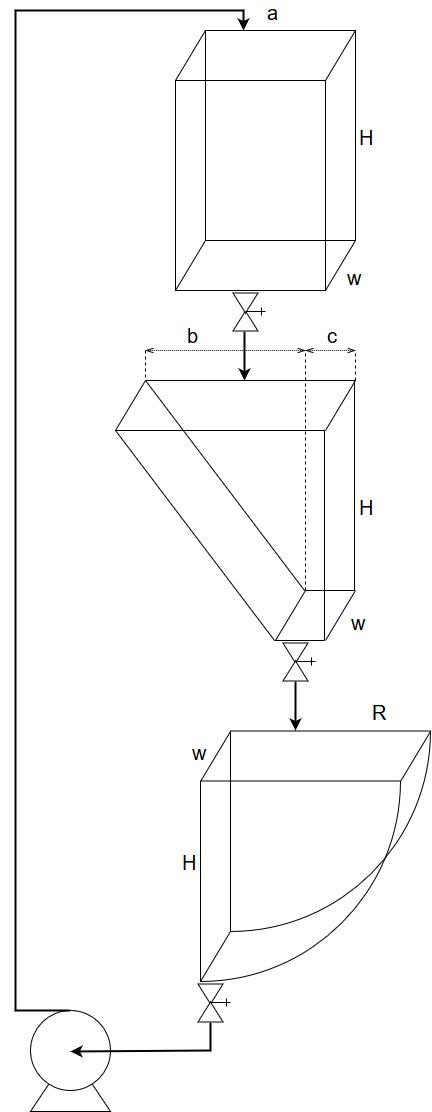
\includegraphics[scale=.5]{Grafika/schemat_zbiornikow}
	\caption{Układ zbiorników z zaznaczonymi wymiarami}\label{fig:zbiorniki}
\end{figure}

\section{Wprowadzenie z zakresu dynamiki płynów}
\label{sec:plyny}

W niniejszym podrozdziale zostały przypomniane podstawowe prawa fizyki związane z przepływem cieczy oraz jego związkiem z poziomem tej cieczy w zbiorniku.

%-------------------------------------------------
\subsection{Równanie Bernoulliego i prawo Torricellego}
\label{sub:plyny-torr}

Równanie Bernoulliego jest jednym z podstawowych praw termodynamiki płynów idealnych. Mówi ono, że wzrost prędkości przepływu cieczy musi wiązać się ze spadkiem ciśnienia lub energii potencjalnej.
Ma kilka postaci; najpopularniejszą jest tzw. szczególne równanie Bernoulliego, które wiąże energię mechaniczną płynu z jego prędkością w danym miejscu, wysokością w układzie odniesienia służącym do wyznaczania energii potencjalnej, ciśnieniem i gęstością.
W takiej formie można je stosować tylko do cieczy nieściśliwych i nielepkich, jednocześnie zakładając stacjonarność i bezwirowość przepływu.

Ta szczególna postać równania Bernoulliego jest przedstawiona jako równanie \ref{eq:bernoulli}.

\begin{equation}\label{eq:bernoulli}
e_{m} = \frac{v^2}{2} + gh + \frac{p}{\rho} = const
\end{equation}

Oznaczenia:
\begin{itemize}
	\item $e_{m}$ - energia jednostki masy cieczy,
	\item $v$ - prędkość cieczy w danym miejscu,
	\item $g$ - przyspieszenie grawitacyjne,
	\item $h$ - wysokość w układzie odniesienia, w którym jest wyznaczana energia potencjalna,
	\item $p$ - ciśnienie cieczy w danym miejscu,
	\item $\rho$ - gęstość cieczy.
\end{itemize}

Z równania Bernoulliego można wyprowadzić bezpośrednią zależność między prędkością cieczy a jej poziomem w zbiorniku. Jest ona znana pod nazwą prawa Torricellego i przedstawiona jako równanie \ref{eq:torricelli} (przyjęto oznaczenia takie jak w przypadku równania \ref{eq:bernoulli}).
Można owo prawo zapisać w bardziej ogólnej formie słownej:

\begin{torricelli}
    Prędkość wypływu cieczy jest proporcjonalna do pierwiastka kwadratowego z poziomu cieczy w zbiorniku.
    \begin{equation}\label{eq:torricelli}
    v = \sqrt{2gh}
    \end{equation}
\end{torricelli}
Takie sformułowanie tego prawa będzie istotne w dalszych krokach wyznaczania modelu matematycznego rozważanego układu.


\subsection{Bilans masy}
\label{sub:plyny-bilans}

Kolejnym zjawiskiem fizycznym, którego zrozumienie jest potrzebne, aby wyznaczyć model matematyczny rozważanego w niniejszej pracy układu zbiorników, jest bilans masy, czyli bezpośrednia konsekwencja \emph{prawa zachowania masy}.

\begin{mass}
    Masa układu ciał (suma mas wszystkich ciał wchodzących w skład tego układu) nie zmienia się podczas przemian i oddziaływań fizycznych w nim zachodzących.
    \begin{equation}\label{eq:mass-conservation}
        m_{uk} = const
    \end{equation}
\end{mass}

Rozważając układ pojedynczego zbiornika z cieczą, do którego ta ciecz jest nalewana i z którego się ona wylewa, można sformułować następstwo tego prawa dane równaniem \ref{eq:mass-balance}. Mówi ono, że zmiana masy w rozważanym zbiorniku - $m_{zb}$ - jest równa zmianie masy do niego wpływającej - $m_{we}$ - i wypływającej - $m_{wy}$.

\begin{equation}\label{eq:mass-balance}
    \frac{\partial m_{we}}{\partial t} - \frac{\partial m_{wy}}{\partial t} =\frac{\partial m_{zb}}{\partial t}
\end{equation}

Przyjmując założenie, że ciecz w zbiorniku i poza nim ma stałą gęstość $\rho$ oraz stosując następujące podstawienia:
\begin{itemize}
    \item $m_{zb} = V_{zb}\cdot\rho$, gdzie $V_{zb}$ to objętość cieczy w zbiorniku,
    \item $V_{zb} = A_{zb} \cdot h_{zb}$, gdzie $A_{zb}$ to pole przekroju poprzecznego zbiornika, a $h_{zb}$ to wysokość słupa cieczy w tym zbiorniku
\end{itemize}
można przedstawić powyższą zależność w postaci opisanej zależnością \ref{eq:tank-mass-balance} (za: \cite{Postlethwaite}).

\begin{equation}\label{eq:tank-mass-balance}
    A_{zb} \cdot \frac{\partial h_{zb}}{\partial t} = \frac{\partial V_{we}}{\partial t} - \frac{\partial V_{wy}}{\partial t}
\end{equation}

Strumień (zmiana objętości cieczy w czasie) wypływający z takiego zbiornika można otrzymać na podstawie prawa Torricellego - jest on dany zależnością \ref{eq:tank-outflow}, gdzie $C$ to stała proporcjonalności wypływu. W rozważanym układzie będzie on zależeć od ustawienia zaworu wyjściowego z danego zbiornika, a więc można powiedzieć, że strumień opisuje opór wypływu ze zbiornika (za: \cite{TanksManual}).

\begin{equation}\label{eq:tank-outflow}
\frac{\partial V_{wy}}{\partial t} = C\cdot\sqrt{h_{zb}}
\end{equation}

Jeśli chodzi o strumień wpływający, to dla drugiego i trzeciego zbiornika jest on równy strumieniowi wypływającemu z poprzedniego zbiornika. Można przyjąć, że dla pierwszego zbiornika ten strumień to sterowanie pompą. Będzie ono oznaczone symbolem $u$.

Pola powierzchni przekrojów poprzecznych wszystkich trzech zbiorników przedstawiono jako równanie \ref{eq:model-fields}. Zastosowano oznaczenia z \ref{fig:zbiorniki}.

\begin{equation}\label{eq:model-fields}
    \begin{array}{lr}
        A_{1} = w \cdot a \\
        A_{2} = c\cdot w + \frac{h_{2}}{h_{max}}\cdot b\cdot w \\
        A_{3} = w\cdot \sqrt{R^{2} - (R - h_{3})^{2}}
    \end{array}
\end{equation}

%-------------------------------------------------
\subsection{Rodzaje przepływów}
\label{sub:plyny-przeplywy}

Przytoczona wcześniej szczególna postać równania Bernoulliego (równanie \ref{eq:bernoulli}) jest obwarowana założeniem stacjonarności przepływu. Oznacza to dwie rzeczy:
\begin{enumerate}
    \item Wartości wektorów prędkości cieczy są stałe w czasie.
    \item Poszczególne ,,warstwy'' cieczy nie wpływają na siebie.
\end{enumerate}

Drugi z tych warunków jest znany pod nazwą przepływu laminarnego, który zwykle ma miejsce przy niskich prędkościach cieczy. W takim typie przepływu nie występują żadne jego zaburzenia (ruchy wirowe, prądy przeciwne itp.), a zachowanie poszczególnych ,,warstw'' cieczy porównać można do tasowania kart: przepływają obok siebie bez wpływania jedna na drugą. Jej cząstki będące blisko powierzchni przemieszczają się po liniach równoległych do tafli cieczy.

Niestety, w rzeczywistości ciężko jest spełnić założenie laminarności przepływu, nie mówiąc już o jego stacjonarności. W związku z tym można zastosować pewne praktyczne uogólnienie zależności \ref{eq:tank-outflow} w stosunku do cieczy wypływających w sposób nielaminarny. Polega ono na zastąpieniu pierwiastka we wspomnianym wzorze parametrem $\alpha$, którego wartość można dobrać na podstawie pomiarów w rzeczywistym układzie (przykład podany w \cite{TanksManual}). Uwzględniają to uogólnienie, można zapisać nowe sformułowanie zależności \ref{eq:tank-outflow} jako równanie \ref{eq:tank-outflow-nonlmnr}.

\begin{equation}\label{eq:tank-outflow-nonlmnr}
    \frac{\partial V_{wy}}{\partial t} = C\cdot h_{zb}^{\alpha}
\end{equation}


\section{Model matematyczny zestawu zbiorników}
\label{sec:model}

Na podstawie podanych wcześniej zależności można zdefiniować model matematyczny rozważanego układu zbiorników.
Jest on dany równaniem \ref{eq:model} (za: \cite{TanksManual}).

\begin{equation}\label{eq:model}
\left \{
\begin{array}{lr}
\frac{\partial h_{1}}{\partial t} = \frac{u - C_{1}{h_{1}}^{\alpha_{1}}}{aw} \\[8pt]
\frac{\partial h_{2}}{\partial t} = \frac{C_{1}{h_{1}}^{\alpha_{1}} -  C_{2}{h_{2}}^{\alpha_{2}}}{cw + \frac{h_{2}}{h_{max}}bw} \\[12pt]
\frac{\partial h_{3}}{\partial t} = \frac{C_{2}{h_{2}}^{\alpha_{2}} -  C_{3}{h_{3}}^{\alpha_{3}}}{w\sqrt{R^{2} - (R - h_{3})^{2}}}
\end{array}
\right.
\end{equation}

Oznaczenia:
\begin{itemize}
    \item $h(t) = [h_{1}(t)~ h_{2}(t)~ h_{3}(t)]^{T}$ - poziomy wody w zbiornikach,
    \item $u(t)$ - sterowanie pompą,
    \item $a$ - szerokość pierwszego zbiornika,
    \item $b$ - szerokość trójkątnej części drugiego zbiornika,
    \item $c$ - szerokość prostopadłościennej części drugiego zbiornika,
    \item $R$ - promień trzeciego zbiornika,
    \item $w$ - głębokość zbiorników,
    \item $h_{max}$ maksymalna wysokość słupa wody w zbiornikach,
    \item $C_{i}$ - opór wypływu z $i$-tego zbiornika,
    \item $\alpha_{i}$ - współczynnik wypływu z $i$-tego zbiornika.
\end{itemize}

Wszystkie wymiary w powyższym wzorze zostały przedstawione na rys. \ref{fig:zbiorniki}. Są na nim również oznaczone opory wypływów $C_{1}$ - $C_{3}$ przy odpowiednich zaworach.

Przyjmując $\alpha_{i} = \frac{1}{2}, \forall_{i \in \{1, 2, 3\}}$, można uszczegółowić powyższy model, zakładając tylko przepływ laminarny.
Taka właśnie jego postać będzie wykorzystywana przy analitycznym wyznaczeniu współczynników równania sprzężonego (definicja znajduje się w sekcji \ref{sub:toc-def-intro}), które jest przeprowadzone w podrozdziale \ref{sub:toc-ctrl}.
W rzeczywistości, jak zostało wspomniane w podrozdziale \ref{sub:plyny-przeplywy}, wartości tych współczynników będą musiały być trochę mniejsze, aby oddać faktyczny sposób przepływu wody między zbiornikami.

W rozważanym układzie zbiorników przyjmuje się następujące ograniczenia (pomijając oczywiste $t \geq 0$):
\begin{itemize}
    \item ograniczenia równościowe:
    \begin{equation}\label{eq:model-eq-const}
    \begin{array}{lr}
        h_{1}(0) = h_{10}\\
        h_{2}(0) = h_{20}\\
        h_{3}(0) = h_{30}\\
    \end{array}
    \end{equation}
    \item ograniczenia nierównościowe:
    \begin{equation}\label{eq:model-noneq-const}
    \begin{array}{lr}
        \forall_{t \in [0, T]}:~ 0 \leq h_{1}(t) \leq h_{max}\\
        \forall_{t \in [0, T]}:~ 0 \leq h_{2}(t) \leq h_{max}\\
        \forall_{t \in [0, T]}:~ 0 \leq h_{3}(t) \leq h_{max}\\
        \forall_{t \in [0, T]}:~ 0 \leq u(t) \leq u_{max}
    \end{array}
    \end{equation}
\end{itemize}
Parametry $h_{10}$, $h_{20}$ i $h_{30}$ oraz $h_{max}$ traktuje się jako zadane.

Punkty równowagi (nazywane również stanami ustalonymi) takiego systemu będą opisane przez zależność \ref{eq:steady-state-def-model} i wyznaczone przez parę wektora wartości zmiennych stanu $h_{r}$ oraz sterowania $u_{r}$. Brak zależności od czasu owej pary został odpowiednio odnotowany.

\begin{equation}\label{eq:steady-state-def-model}
\frac{\partial h(t)}{\partial t} = 0 ~\Rightarrow~ 
\left \{
\begin{array}{lr}
    \frac{\partial h_{1}}{\partial t} = 0 \\
    \frac{\partial h_{2}}{\partial t} = 0 \\
    \frac{\partial h_{3}}{\partial t} = 0
\end{array}
\right.
\end{equation}

Dla rozważanego układu zbiorników będą miały postać daną zależnością \ref{eq:model-steady-state}.

\begin{equation}\label{eq:model-steady-state}
\begin{array}{lr}
u_{r} = C_{1}h_{1}^{\alpha_{1}} = C_{2}h_{2}^{\alpha_{2}} = C_{3}h_{3}^{\alpha_{3}}\\
h_{r} = \begin{bmatrix}
h_{1r}\\h_{2r}\\h_{3r}
\end{bmatrix}
=
\begin{bmatrix}
\big( \frac{\textstyle u_{r}}{\textstyle C_{1}}\big)^{\frac{\scriptstyle 1}{\scriptstyle \alpha_{1}}}\\
\big( \frac{\textstyle u_{r}}{\textstyle C_{2}}\big)^{\frac{\scriptstyle 1}{\scriptstyle \alpha_{2}}}\\
\big( \frac{\textstyle u_{r}}{\textstyle C_{3}}\big)^{\frac{\scriptstyle 1}{\scriptstyle \alpha_{3}}}
\end{bmatrix}
\end{array}
\end{equation}

Wynika z tego, że układ otwarty jest asymptotycznie stabilny, gdyż posiada tylko jeden, zerowy punkt równowagi (pokazany jako wzór \ref{eq:model-zero-state}). Jest to również zgodne z fizyczną naturą tego systemu zbiorników: przy braku zasilania go pompą, cała woda wycieknie ze wszystkich trzech zbiorników.

\begin{equation}\label{eq:model-zero-state}
h_{r}^{0} = \begin{bmatrix}
h_{1r}^{0}\\h_{2r}^{0}\\h_{3r}^{0}
\end{bmatrix} = 
\begin{bmatrix}
0\\0\\0
\end{bmatrix}
\end{equation}


\section{Regulacja czasooptymalna}
\label{sec:toc}

W niniejszym podrozdziale przedstawiona zostanie koncepcja regulacji czasooptymalnej. Zostaną podane założenia zagadnienia, twierdzenia, na których podstawie można wyliczyć rozwiązanie oraz jego proponowana forma analityczna.

Zaznacza się, że mimo iż podane niżej definicje i założenia są wzięte z ogólnych zagadnień optymalizacji dynamicznej, to w podanym brzmieniu stosują się tylko do zagadnienia wyznaczania sterowania czasooptymalnego.

%-------------------------------------------------
\subsection{Ogólna definicja zagadnienia}
\label{sub:toc-def}

%-------------------
\subsubsection{Założenia wstępne}
\label{sub:toc-def-intro}
Przyjmijmy system dany stacjonarnym, zwyczajnym równaniem różniczkowym (pokazanym jako równanie \ref{eq:general_system}), w którym:

\begin{equation}\label{eq:general_system}
    \frac{\partial x(t)}{\partial t} = f(x(t), u(t)), ~ 0 \leq t \leq T
\end{equation}

\begin{itemize}
    \item wektor zmiennych stanu w chwili $t$ - $x(t)$ spełnia następujące założenia:
    \begin{itemize}
        \item $\forall_{t \geq 0}:~ x(t) \in \mathbb{R}^{n}$ - ma $n$ składowych, a więc rozważany system ma $n$ równań różniczkowych zwyczajnych,
        \item $x(0) = x_{0} \in \mathbb{R}^{n}$ - spełnia warunek początkowy $x_{0}$;
    \end{itemize}
    \item wektor sterowań w chwili $t$ - $u(t)$:
    \begin{itemize}
        \item $\forall_{t \geq 0}:~ u(t) \in D \subset \mathbb{R}^{m}$ - ma $m$ składowych zawierającym się w zbiorze $D$ ograniczającym wartości sterowań,
        \item $u(0) = u_{0}$ - spełnia warunek początkowy $u_{0}$,
        \item funkcja $u$ jest przedziałami ciągła na przedziale $[0, T]$, czyli:
        \begin{itemize}
            \item ma co najwyżej skończoną liczbę punktów nieciągłości,
            \item w każdym z nich ma skończoną granicę lewostronną,
            \item jest prawostronnie ciągła,
            \item w lewym końcu przedziału jest lewostronnie ciągła;
        \end{itemize}
    \end{itemize}
    \item funkcja $f: \mathbb{R}^{n} \times \mathbb{R}^{m} \longmapsto \mathbb{R}^{n}$:
    \begin{itemize}
        \item $f \in C^{1}$ - jest ciągła i różniczkowalna ze względu na pierwszy argument,
        \item $\frac{\partial f(t)}{\partial x} \in C^{0}$ - jej pochodna ze względu na pierwszy argument jest ciągła.
    \end{itemize}
\end{itemize}

Rozwiązaniem takiego równania jest oczywiście funkcja $x: [0, T) \longmapsto \mathbb{R}^{n}$ nazywana \emph{trajektorią układu}.

Trajektoria będąca rozwiązaniem zagadnienia minimalnoczasowego musi spełniać następujący warunek końcowy (nazywany również stanem docelowym):
\begin{equation}\label{eq:final_term}
    x(T) = x_{f} \in \mathbb{R}^{n}
\end{equation}

Ów czas $T$, po którym przy danym sterowaniu stan systemu osiągnie warunek końcowy, będzie wskaźnikiem jakości: 
\begin{equation}\label{eq:quality}
    Q(u(t)) = q(x_{f}) = T
\end{equation}

Na tej podstawie można określić \emph{sterowanie optymalne} $\hat{u}(t)$, które spełnia wszystkie wspominane przy opisie równania \ref{eq:general_system} warunki oraz zależność \ref{eq:optimal_quality}. Trajektoria układu wygenerowana przez zastosowanie sterowania optymalnego nazwana jest \emph{trajektorią optymalną} i opisana symbolem $\hat{x}(t)$.
\begin{equation}\label{eq:optimal_quality}
    \forall_{u(t)}:~ Q(u(t)) \leq Q(\hat{u}(t))
\end{equation}

W opisie zagadnienia czasooptymalnego potrzebne są jeszcze dwa pojęcia.
Pierwsze to \emph{funkcja sprzężona} $\psi: [0, T] \longmapsto \mathbb{R}^{n}$ będąca rozwiązaniem tzw. równania sprzężonego \ref{eq:costate-def}.
\begin{equation}\label{eq:costate-def}
\frac{\partial \psi(t)}{\partial t} = - \frac{\partial f(x(t), u(t)}{\partial x}
\end{equation}

Tak, jak w przypadku trajektorii optymalnej układu, trajektoria $\psi(t)$ wyznaczona w układzie, w którym zastosowane zostało sterowanie optymalne $\hat{u}(t)$, nosi nazwę \emph{trajektorii sprzężonej optymalnej} i oznaczona jest symbolem $\hat{\psi}(t)$.

Ostatnim pojęciem potrzebnym w niniejszym zagadnieniu jest \emph{hamiltonian}, zwany również \emph{funkcją Hamiltona}, czyli funkcja $H: \mathbb{R}^{n} \times \mathbb{R}^{n} \times \mathbb{R}^{m} \longmapsto \mathbb{R}$ który dla trajektorii układu $x(t)$ wygenerowanej przy pomocy sterowania $u(t)$ i odpowiadającej im trajektorii sprzężonej $\psi(t)$ zdefiniowany jest zależnością \ref{eq:hamiltonian-def}.

\begin{equation}\label{eq:hamiltonian-def}
H(\psi(t), x(t), u(t)) = \psi(t) \circ f(x(t), u(t)) = \psi(t)^{T} \cdot f(x(t), u(t))
\end{equation}

%-------------------
\subsubsection{Zasada maksimum Pontriagina}
\label{sub:toc-def-pontriagin}

Aby jednoznacznie opisać, a następnie wyznaczyć sterowanie czasooptymalne, potrzebne jest przytoczenie zasadniczego twierdzenia w optymalizacji dynamicznej. Jest ono znane pod nazwą \emph{zasada maksimum Pontriagina}. Zostało opracowane w 1956 r. przez rosyjskiego matematyka Lwa Pontriagina.

\begin{pontriagin-max}\label{the:pontryagin}
    Zakładając układ opisany równaniem \ref{eq:general_system} z warunkiem końcowym \ref{eq:final_term} i wskaźnikiem jakości \ref{eq:quality} oraz równanie sprzężone \ref{eq:costate-def}:\\
    jeśli dla trajektorii układu $\hat{x}(t)$ wygenerowanej przy pomocy sterowania $\hat{u}(t)$ i odpowiadającej im trajektorii sprzężonej $\hat{\psi}(t)$ zachodzi:\\
    \begin{equation}\label{eq:pontriagin}
    \forall_{u(t) \in D}~ \forall_{t \in [0, T]}:~ H(\hat{\psi}(t), \hat{x}(t), \hat{u}(t)) ~ \geq ~ H(\hat{\psi}(t), \hat{x}(t), u(t))
    \end{equation}
    to sterowanie $\hat{u}(t)$ jest sterowaniem optymalnym.
\end{pontriagin-max}

Powyższe twierdzenie należy obwarować dodatkowymi warunkami koniecznymi optymalności. Niech funkcja $g: \mathbb{R}^{2n} \longmapsto \mathbb{R}^{l}$ opisuje zestaw ograniczeń nierównościowych, a funkcja $h: \mathbb{R}^{2n} \longmapsto \mathbb{R}^{k}$ - ograniczeń równościowych. Obie dane są wzorem \ref{eq:pontryagin-constraints}. Dodatkowo zakłada się, że $g, h \in C^{1}$.
\begin{equation}\label{eq:pontryagin-constraints}
    \begin{array}{lr}
    g(x_{0}, x_{f}) \leq 0 \\
    h(x_{0}, x_{f}) = 0
    \end{array}
\end{equation}

Ponadto, zakłada się, że istnieją $\lambda \in \mathbb{R}$, $\mu \in \mathbb{R}^{l}$ oraz $\rho \in \mathbb{R}^{k}$, które wraz z uprzednio zdefiniowanymi wielkościami i funkcjami spełniają następujące \emph{warunki konieczne optymalności}:
\begin{itemize}
    \item warunek nieujemności:
    \begin{equation}\label{eq:pontryagin-noneg}
    \lambda \geq 0 \land \|\mu\| \geq 0
    \end{equation}
    \item warunek nietrywialności:
    \begin{equation}\label{eq:pontryagin-notriv}
    \lambda + \|\mu\| + \|\rho\| > 0
    \end{equation}
    \item warunek komplementarności:
    \begin{equation}\label{eq:pontryagin-comp}
    \mu \circ g(x_{0}, x_{f}) = 0
    \end{equation}
    \item warunki transwersalności:
    \begin{equation}\label{eq:pontryagin-trans}
    \begin{array}{lr}
        \hat{\psi}(0) = \frac{\partial (\mu \circ g + \rho \circ h)}{\partial x_{0}}\\[8pt]
        \hat{\psi}(T) = - \frac{\partial (\mu \circ g + \rho \circ h)}{\partial x_{f}}\\[8pt]
        \forall_{t \in [0, T]}:~ H(\psi(t), x(t), u(t)) = \frac{\partial (\lambda T + \mu \circ g + \rho \circ h)}{\partial T} = \lambda
    \end{array}
    \end{equation}
    \item równanie sprzężone dane wzorem \ref{eq:costate-def},
    \item warunek maksimum hamiltonianu dany wzorem \ref{eq:pontriagin}.
\end{itemize}

%-------------------------------------------------
\subsection{Wyznaczanie sterowania czasooptymalnego}
\label{sub:toc-ctrl}

Analityczne rozwiązania poszukiwania sterowania czasooptymalnego zwykle opierają się bezpośrednio na przytoczonej powyżej zasadzie maksimum i warunkach koniecznych optymalności. W niniejszym podrozdziale zostanie pokrótce przedstawiona droga mogąca zmierzać do wyznaczenia analitycznego czasooptymalnego sterowania w rozważanym układzie zbiorników. Całe rozwiązanie nie jest przeprowadzone ze względu na fakt, iż równiania sprzężone są niestacjonarne, a więc ich rozwiązanie analityczne byłoby bardzo trudne lub wręcz niemożliwe.

Aby dodatkowo uprościć analizę problemu oraz fizyczne zastosowanie wyznaczonego sterowania, zakłada się, że poszukiwane jego postaci będą klasy "bang - bang". To znaczy, że będą przyjmowały tylko wartości z brzegów zbioru dopuszczalnego $D$. Można przyjąć takie założenie, ze względu na to, iż:
\begin{itemize}
    \item sterowanie $u$ jest jednowymiarowe: $D \in \mathbb{R} \Rightarrow D = [0, u_{max}]$,
    \item %TODO: dopisać dlaczego można stosować sterowanie bang-bang
\end{itemize}

Pierwszym krokiem ku wyliczeniu analitycznego rozwiązania jest wyznaczenie równań sprzężonych za pomocą wzoru \ref{eq:costate-def}. Przyjmując współczynniki $\alpha_{i} = \frac{1}{2} \forall_{i \in \{1, 2, 3\}}$ w modelu matematycznym zestawu zbiorników danym równaniem \ref{eq:model}, można wyznaczyć równania sprzężone rozważanego układu. Są one dane wzorem \ref{eq:sprzezone}. Pominięto w nim zależności wszystkich funkcji $\psi$ oraz $h$ od czasu, aby uprościć zapis.

\begin{equation}\label{eq:sprzezone}
	\left \{
	\begin{array}{lr}
		\frac{\partial \psi_{1}}{\partial t} =  \psi_{1}\frac{C_{1}}{2aw\sqrt{h_{1}}} - \psi_{2}\frac{C_{1}}{2\sqrt{h_{1}}(cw + \frac{h_{2}}{h_{max}}bw)} \\[20pt]
		\frac{\partial \psi_{2}}{\partial t} = - \psi_{2}\frac{1}{cw + \frac{h_{2}}{h_{max}}bw}(\frac{b(C_{1}\sqrt{h_{1}} - C_{2}\sqrt{h_{2}})}{ch_{max} + bh_{2}} - \frac{C_{2}}{2\sqrt{h_{2}}}) - \psi_{3}\frac{1}{w\sqrt{h_{3}(2R - h_{3})}} \\[20pt]
		\frac{\partial \psi_{3}}{\partial t} = \psi_{3}\frac{-C_{3}(3R - 2h_{3})}{wh_{3}(2R - h_{3})^{\frac{3}{2}}}
	\end{array}
	\right.
\end{equation}

Następnie trzeba by przedefiniować ograniczenia równościowe (dane wzorem \ref{eq:model-eq-const}) i nierównościowe (\ref{eq:model-noneq-const}) tak, aby spełniały założenia funkcji $g$ i $h$ opisane zależnościami \ref{eq:pontryagin-constraints}.
Korzystając z warunków komplementarności (\ref{eq:pontryagin-comp}) oraz nieujemności (\ref{eq:pontryagin-noneg}), powinno się wyznaczyć składowe wektora $\mu$ oraz założyć pewną postać wektora $\rho$.
%TODO: sprawdzic, czy rzeczywiście nie da się wyznaczyć 

Na podstawie tych danych należałoby wyznaczyć warunki początkowy i końcowy danym wzorem \ref{eq:pontryagin-trans} dla powyższych równań sprzężonych, co pozwoliłoby wyznaczyć analityczne wzory opisujące wszystkie składowe trajektorii sprzężonych systemu.


%-------------------------------------------------
\subsection{Nieliniowość układu a sterowanie czasooptymalne}
\label{sub:toc-nonlnr}


%-------------------------------------------------
\subsection{Numeryczne metody wyznaczania sterowania czasooptymalnego}
\label{sub:toc-num}

\section{Regulacja liniowo - kwadratowa}
\label{sec:lqr}

W niniejszym podrozdziale zostanie przedstawione zagadnienie szukania sterowania w układach liniowych z tzw. liniowo-kwadratowym wskaźnikiem jakości. Pokazana zostanie również metoda zastosowania takiego typu regulacji dla układów nieliniowych przy użyciu linearyzacji w punkcie pracy.

%-------------------------------------------------
\subsection{Ogólna definicja zagadnienia}
\label{sub:lqr-def}


%-------------------------------------------------
\subsection{Linearyzacja modelu}
\label{sub:lqr-lin}


%-------------------------------------------------
\subsection{Wyznaczanie regulatora liniowo - kwadratowego}
\label{sub:lqr-ctrl}


%-------------------------------------------------
\subsection{Dobór wag w zagadnieniu liniowo - kwadratowym}
\label{sub:lqr-weights}

\chapter{Architektura zaproponowanego rozwiązania}
\label{cha:arch}

W niniejszej pracy została zaproponowana hybrydowa struktura aplikacji realizującej zadania wyliczania i aplikowania sterowania czasooptymalnego, jak i minimalnego w sensie liniowo-kwadratowego wskaźnika jakości.
Taka jej architektura jest odbiciem faktycznej tendencji w automatyce ostatnich lat: aby skomplikowane zadania obliczeniowe zadawać nie tym elementom, które realizują bezpośrednie sterowanie, ale zlecać je innym urządzeniom o architekturze sprzętu odpowiedniejszej do radzenia sobie z takimi problemami.

Dokładnie takie podejście zostało również zaprezentowane w niniejszej pracy. Hybrydowa (z łaciny: \emph{hybrida}: mieszaniec, krzyżówka) struktura polega na zastosowaniu dwóch poziomów: obliczeniowego i realizującego sterowanie bezpośrednie. Zostały one szerzej opisane w tym rozdziale.

\section{Podział zadań między elementami oprogramowania}
\label{sec:podzial-zadan}

W związku z zaproponowaną w niniejszej pracy architekturą oprogramowania, opierającą się na dwóch poziomach, kluczowym aspektem tego opracowania jest odpowiedni podział zadań między tymi poziomami.

Pierwszy z nich to część ,,wyższego poziomu'' - została tak określona ze względu na to, iż nie ma bezpośredniego wpływu na kontrolowany fizyczny obiekt, a zajmuje się tylko modelem matematycznym. Jej zadania są przedstawione na poniższej liście.

\begin{enumerate}
    \item Symulacja modelu nieliniowego w pętli otwartej, aby zainicjować algorytm optymalizacji dynamicznej.
    \item Wyznaczanie sterowania czasooptymalnego dla zadanych wartości początkowych i końcowych.
    \item Symulacja modelu nieliniowego w pętli zamkniętej, aby zweryfikować wyliczone sterowanie czasooptymalne.
    \item Linearyzacja modelu w punkcie pracy.
    \item Wyznaczanie sterowania optymalnego w sensie liniowo-kwadratowego wskaźnika jakości (dla modelu linearyzowanego w punkcie pracy).
\end{enumerate}

Dodatkowo przyjęto następujące założenia w związku z tymi zadaniami (podzielone ze względu na to, którego zagadnienia optymalizacji dotyczą):

\begin{enumerate}
    \item Założenia związane ze sterowaniem czasooptymalnym:
    \begin{enumerate}
        \item Sterowanie czasooptymalne jest postaci ,,bang-bang'' (wyjaśnienie w sekcji \ref{sub:toc-nonlnr}).
        \item W związku z tym wystarczy wyznaczyć czasy przełączeń między konkretnymi sterowaniami maksymalnym i minimalnym oraz to, które z nich ma być aplikowane jako pierwsze.
    \end{enumerate}
    \item Założenia związane ze sterowaniem liniowo-kwadratowym:
    \begin{enumerate}
        \item Punkt pracy (w którym jest dokonywana linearyzacja) jest stanem docelowym zagadnienia czasooptymalnego, jeśli ten jest punktem równowagi systemu (definicja dana w podrozdziale \ref{sec:model}).
        \item Jeśli stan docelowy zagadnienia czasooptymalnego nie jest stanem ustalonym rozważanego układu, stosuje się przybliżenie go do pewnego punktu równowagi i tam dokonuje się linearyzacji modelu matematycznego.
        \item Sterowanie liniowo-kwadratowe jest wyliczane jako odchyłka od sterowania ustalonego dla punktu równowagi.
    \end{enumerate}
\end{enumerate}

Na podstawie powyższych zadań oraz założeń sformułowano poniższą listę parametrów, które musi przyjmować część optymalizacyjna od użytkownika:

\begin{itemize}
    \item parametry statyczne modelu matematycznego:
    \begin{itemize}
        \item fizyczne rozmiary zbiorników (parametry $a$, $b$, $c$, $R$, $w$ i $h_{max}$),
        \item opory wypływu ze zbiorników (parametry $C_{1}$, $C_{2}$ oraz $C_{3}$),
        \item współczynniki wypływu ze zbiorników(parametry $\alpha_{1}$, $\alpha_{2}$ i $\alpha_{3}$);
    \end{itemize}
    \item wielkości związane z ograniczeniami w zagadnieniu czasooptymalnym:
    \begin{itemize}
        \item maksymalne sterowanie ($u_{max}$),
        \item wartości początkowe poziomów wody w zbiornikach (parametry $h_{10}$, $h_{20}$ oraz $h_{30}$),
        \item wartości końcowe poziomów wody w zbiornikach (parametry $h_{1f}$, $h_{2f}$ i $h_{3f}$);
    \end{itemize}
    \item wagi w zagadnieniu liniowo-kwadratowym:
    \begin{itemize}
        \item wartość wagi sterowania $R \in \mathbb{R}$,
        \item wartości wag stanów dane jako macierz $Q \in \mathbb{R}^{3}$.
    \end{itemize}
\end{itemize}

Drugi poziom zaproponowanego w niniejszej pracy rozwiązania to część ,,niższego poziomu'' - jej nazwa jest związana z tym, że bezpośrednio wpływa na sterowany układ. Nie zawiera tak skomplikowanych narzędzi obliczeniowych, ale za to powinna cechować się dużą niezawodnością. Jej zadania są przedstawione na poniższej liście.

\begin{enumerate}
    \item Aplikacja sterowania czasooptymalnego przez czas, który jest wyliczony przez część ,,wyższego poziomu'' oraz w odpowiedniej postaci (,,bang-bang'').
    \item Po upływie tego czasu aplikacja sterowania optymalnego w sensie liniowo-kwadratowego wskaźnika jakości aż do czasu otrzymania kolejnego sterowania czasooptymalnego.
    \item Symulacja układu modelu matematycznego w celach testowych i weryfikacyjnych.
\end{enumerate}

W związku z tym, że jest to element realizujący bezpośrednie sterowanie, użytkownik nie powinien mieć wpływu na jego funkcjonowanie. Cały interfejs między nim a programem sterującym powinien dotyczyć tylko i wyłącznie części ,,wyższego poziomu''.


\section{Część obliczeniowa (,,wyższego poziomu'')}
\label{sec:czesc-wyzsza}


%-------------------------------------------------
\subsection{Wybór pakietu do optymalizacji dynamicznej}
\label{sub:czesc-wyzsza-wybor}


%-------------------------------------------------
\subsection{Opis pakietu Modelica}
\label{sub:czesc-wyzsza-modelica}


%-------------------------------------------------
\subsection{Opis systemu Tango Controls}
\label{sub:czesc-wyzsza-tango}


%-------------------------------------------------
\subsection{Architektura klasy urządzeń systemu Tango}
\label{sub:czesc-wyzsza-klasa}


\subsubsection{Interfejs dla systemu Tango}


\subsubsection{Problem dostępności interfejsu}


%-------------------------------------------------
\subsection{Środowisko testowe części obliczeniowej}
\label{sub:czesc-wyzsza-docker}

\section{Część realizująca sterowanie ("niższego poziomu")}
\label{sec:czesc-nizsza}


%-------------------------------------------------
\subsection{Pakiet Simulink jako narzędzie realizujące sterowanie}
\label{sub:czesc-nizsza-matlab}


%-------------------------------------------------
\subsection{Komunikacja z urządzeniem wykonawczym i czujnikami}
\label{sub:czesc-nizsza-komunikacja}


\section{Komunikacja między elementami oprogramowania}
\label{sec:komunikacja}



\chapter{Badania symulacyjne}
\label{cha:symulacja}

\section{Optymalizacja przy użyciu pakietu \texttt{JModelica.org}}
\label{sec:opt}


%-------------------------------------------------
\subsection{Inicjalizacja optymalizacji dynamicznej}
\label{sub:opt-init}


%-------------------------------------------------
\subsection{Dokładność wyznaczania rozwiązania}
\label{sub:opt-dokladnosc}


\section{Symulacja i weryfikacja}
\label{sec:sym-wer}


%-------------------------------------------------
\subsection{Przy użyciu pakietu \texttt{JModelica.org}}
\label{sub:sym-wer-jmodelica}


%-------------------------------------------------
\subsection{Przy użyciu oprogramowania MATLAB/Simulink}
\label{sub:sym-wer-matlab}


\chapter{Badania eksperymentalne}
\label{cha:eksperyment}

\section{Porównanie wyników eksperymentalnych z symulacyjnymi}
\label{sec:porownanie}


%-------------------------------------------------
\subsection{Ocena jakości rozwiązania}
\label{sub:porownanie-ocena}


\section{Badanie wpływu zakłóceń na sterowanie}
\label{sec:zaklocenia}


%-------------------------------------------------
\subsection{Wpływ czasu dyskretyzacji}
\label{sub:zaklocenia-dyskretyzacja}


%-------------------------------------------------
\subsection{Wpływ zakłóceń w ruchu sieciowym}
\label{sub:zaklocenia-siec}


\section{Możliwe kierunki dalszego rozwiązania zaproponowanego rozwiązania}
\label{sec:przyszlosc}



\chapter*{Zakończenie}
\addcontentsline{toc}{chapter}{Zakończenie}
\label{cha:zakonczenie}

Przygotowanie aplikacji realizującej postawione we wstępie niniejszej pracy cele okazało się zadaniem tyleż trudnym, co fascynującym. Obie te cechy wynikały przede wszystkim z założeń postawionych przed wyższym poziomem aplikacji opisanych na początku podrozdziału \ref{sec:czesc-wyzsza}. Znalezienie i opisanie otwartego oprogramowania, które potrafi rozwiązywać problemy optymalizacji dynamicznej układów nieliniowych i posiada przystępny interfejs użytkownika, jest niewątpliwą wartością tej pracy.

Udało się zrealizować wszystkie cele: pokazano, iż wyższy poziom aplikacji jest w stanie wyznaczać sterowanie optymalne w rozumieniu dwóch wskaźników jakości: liniowo-kwadratowego i czasowego. Umożliwia on również przeprowadzenie symulacji weryfikacyjnych wyznaczonych sterowań, które opisano w rozdziale \ref{cha:symulacja}. Niższy poziom aplikacji został przygotowany z myślą o komunikacji z układem pomiarowo-sterującym, ale ona nie została przetestowana. Używano tego poziomu tylko w celach symulacyjnych, co dało możliwość sprawdzenia funkcjonowania wyznaczonego sterowania optymalnego poza środowiskiem, w którym zostało obliczone.

Podstawowym kierunkiem dalszych prac byłoby połączenie napisanej aplikacji z rzeczywistym obiektem, co na pewno dostarczyłyby istotnych wniosków co do funkcjonowania całości aplikacji. Byłoby dobrze uzupełnić również opis problemu o identyfikację elementów wykonawczych oraz wyznaczenie zbioru stanów osiągalnych, aby ograniczyć użytkownikowi zbiór możliwych punktów końcowych optymalizacji. Można by również przygotować układ predykcyjny, w celu poprawy błędów sterowania obliczanego w czasie działania aplikacji. Zapewne byłoby to potrzebne przy użyciu jej z rzeczywistym układem zbiorników.

Poza tym należałoby udoskonalić inicjalizację optymalizacji, gdyż to zagadnienie nie zostało rozpoznane dogłębnie w niniejszej pracy. Jest to jednak problem na tyle złożony, że z powodzeniem mógłby stać się tematem kolejnej pracy dyplomowej. Nie testowano również wszystkich możliwości dostosowania algorytmu optymalizacji do potrzeb tego zagadnienia.

%\chapter{Przykłady elementów pracy dyplomowej}

\section{Liczba}

Pakiet \texttt{siunitx} zadba o to, by liczba została poprawnie sformatowana: \\
\begin{center}
	\num{1234567890.0987654321}
\end{center}


\section{Rysunek}

Pakiet \texttt{subcaption} pozwala na umieszczanie w podpisie rysunku odnośników do ,,podilustracji'': \\

\begin{figure}[h]
	\centering
	\begin{subfigure}{0.35\textwidth}
		\centering
		\framebox[2.0\width]{A}
		\subcaption{\label{subfigure_a}}
	\end{subfigure}
	\begin{subfigure}{0.35\textwidth}
		\centering
		\framebox[2.0\width]{B}
		\subcaption{\label{subfigure_b}}
	\end{subfigure}
	
	\caption{\label{fig:subcaption_example}Przykład użycia \texttt{\textbackslash subcaption}: \protect\subref{subfigure_a} litera A, \protect\subref{subfigure_b} litera B.}
\end{figure}

\section{Tabela}

Pakiet \texttt{threeparttable} umożliwia dodanie do tabeli adnotacji: \\

\begin{table}[h]
	\centering
	
	\begin{threeparttable}
		\caption{Przykład tabeli}
		\label{tab:table_example}
		
		\begin{tabularx}{0.6\textwidth}{C{1}}
			\toprule
			\thead{Nagłówek\tnote{a}} \\
			\midrule
			Tekst 1 \\
			Tekst 2 \\
			\bottomrule
		\end{tabularx}
		
		\begin{tablenotes}
			\footnotesize
			\item[a] Jakiś komentarz\textellipsis
		\end{tablenotes}
		
	\end{threeparttable}
\end{table}

\section{Wzory matematyczne}

Czasem zachodzi potrzeba wytłumaczenia znaczenia symboli użytych w równaniu. Można to zrobić z użyciem zdefiniowanego na potrzeby niniejszej klasy środowiska \texttt{eqwhere}.

\begin{equation}
E = mc^2
\end{equation}
gdzie
\begin{eqwhere}[2cm]
	\item[$m$] masa
	\item[$c$] prędkość światła w próżni
\end{eqwhere}

Odległość półpauzy od lewego marginesu należy dobrać pod kątem najdłuższego symbolu (bądź listy symboli) poprzez odpowiednie ustawienie parametru tego środowiska (domyślnie: 2 cm).

%\chapter{Wprowadzenie}
\label{cha:wprowadzenie}

\LaTeX~jest systemem składu umożliwiającym tworzenie dowolnego typu dokumentów (w~szczególności naukowych i technicznych) o wysokiej jakości typograficznej (\cite{Dil00}, \cite{Lam92}). Wysoka jakość składu jest niezależna od rozmiaru dokumentu -- zaczynając od krótkich listów do bardzo grubych książek. \LaTeX~automatyzuje wiele prac związanych ze składaniem dokumentów np.: referencje, cytowania, generowanie spisów (treśli, rysunków, symboli itp.) itd.

\LaTeX~jest zestawem instrukcji umożliwiających autorom skład i wydruk ich prac na najwyższym poziomie typograficznym. Do formatowania dokumentu \LaTeX~stosuje \TeX a (wymiawamy 'tech' -- greckie litery $\tau$, $\epsilon$, $\chi$). Korzystając z~systemu składu \LaTeX~mamy za zadanie przygotować jedynie tekst źródłowy, cały ciężar składania, formatowania dokumentu przejmuje na siebie system.

%---------------------------------------------------------------------------

\section{Cele pracy}
\label{sec:celePracy}


Celem poniższej pracy jest zapoznanie studentów z systemem \LaTeX~w zakresie umożliwiającym im samodzielne, profesjonalne złożenie pracy dyplomowej w systemie \LaTeX.

\subsection{Jakiś tytuł}

\subsubsection{Jakiś tytuł w subsubsection}


\subsection{Jakiś tytuł 2}

%---------------------------------------------------------------------------

\section{Zawartość pracy}
\label{sec:zawartoscPracy}

W rodziale~\ref{cha:pierwszyDokument} przedstawiono podstawowe informacje dotyczące struktury dokumentów w \LaTeX u. Alvis~\cite{Alvis2011} jest językiem 



















%\chapter{Pierwszy dokument}
\label{cha:pierwszyDokument}

W rozdziale tym przedstawiono podstawowe informacje dotyczące struktury prostych plików \LaTeX a. Omówiono również metody kompilacji plików z zastosowaniem programów \emph{latex} oraz \emph{pdflatex}.

%---------------------------------------------------------------------------

\section{Struktura dokumentu}
\label{sec:strukturaDokumentu}

Plik \LaTeX owy jest plikiem tekstowym, który oprócz tekstu zawiera polecenia formatujące ten tekst (analogicznie do języka HTML). Plik składa się z dwóch części:
\begin{enumerate}%[1)]
\item Preambuły -- określającej klasę dokumentu oraz zawierającej m.in. polecenia dołączającej dodatkowe pakiety;

\item Części głównej -- zawierającej zasadniczą treść dokumentu.
\end{enumerate}


\begin{lstlisting}
\documentclass[a4paper,12pt]{article}      % preambuła
\usepackage[polish]{babel}
\usepackage[utf8]{inputenc}
\usepackage[T1]{fontenc}
\usepackage{times}

\begin{document}                           % część główna

\section{Sztuczne życie}

% treść
% ąśężźćńłóĘŚĄŻŹĆŃÓŁ

\end{document}
\end{lstlisting}

Nie ma żadnych przeciwskazań do tworzenia dokumentów w~\LaTeX u w~języku polskim. Plik źródłowy jest zwykłym plikiem tekstowym i~do jego przygotowania można użyć dowolnego edytora tekstów, a~polskie znaki wprowadzać używając prawego klawisza \texttt{Alt}. Jeżeli po kompilacji dokumentu polskie znaki nie są wyświetlane poprawnie, to na 95\% źle określono sposób kodowania znaków (należy zmienić opcje wykorzystywanych pakietów).


%---------------------------------------------------------------------------

\section{Kompilacja}
\label{sec:kompilacja}


Załóżmy, że przygotowany przez nas dokument zapisany jest w pliku \texttt{test.tex}. Kolejno wykonane poniższe polecenia (pod warunkiem, że w pierwszym przypadku nie wykryto błędów i kompilacja zakończyła się sukcesem) pozwalają uzyskać nasz dokument w formacie pdf:
\begin{lstlisting}
latex test.tex
dvips test.dvi -o test.ps
ps2pdf test.ps
\end{lstlisting}
%
lub za pomocą PDF\LaTeX:
\begin{lstlisting}
pdflatex test.tex
\end{lstlisting}

Przy pierwszej kompilacji po zmiane tekstu, dodaniu nowych etykiet itp., \LaTeX~tworzy sobie spis rozdziałów, obrazków, tabel itp., a dopiero przy następnej kompilacji korzysta z tych informacji.

W pierwszym przypadku rysunki powinny być przygotowane w~formacie eps, a~w~drugim w~formacie pdf. Ponadto, jeżeli używamy polecenia \texttt{pdflatex test.tex} można wstawiać grafikę bitową (np. w formacie jpg).



%---------------------------------------------------------------------------

\section{Narzędzia}
\label{sec:narzedzia}


Do przygotowania pliku źródłowego może zostać wykorzystany dowolny edytor tekstowy. Niektóre edytory, np. GEdit, mają wbudowane moduły ułatwiające składanie tekstów w LaTeXu (kolorowanie składni, skrypty kompilacji, itp.).

Jednym z bardziej znanych środowisk do składania dokumentów  \LaTeX a jest {\em TeXstudio}, oferujące kompletne środowisko pracy. Zobacz: \url{http://www.texstudio.org}


Bardzo dobrym środowiskiem jest również edytor gEdit z wtyczką obsługującą \LaTeX a. Jest to standardowy edytor środowiska Gnome. Po instalacji wtyczki obsługującej \LaTeX~ zamienia się w wygodne i szybkie środowisko pracy.

\textbf{Dla testu łamania stron powtórzenia powyższego tekstu.}


Do przygotowania pliku źródłowego może zostać wykorzystany dowolny edytor tekstowy. Niektóre edytory, np. GEdit, mają wbudowane moduły ułatwiające składanie tekstów w LaTeXu (kolorowanie składni, skrypty kompilacji, itp.).
Jednym z bardziej znanych środowisk do składania dokumentów  \LaTeX a jest {\em TeXstudio}, oferujące kompletne środowisko pracy. Zobacz: \url{http://www.texstudio.org}
Bardzo dobrym środowiskiem jest również edytor gEdit z wtyczką obsługującą \LaTeX a. Jest to standardowy edytor środowiska Gnome. Po instalacji wtyczki obsługującej \LaTeX~ zamienia się w wygodne i szybkie środowisko pracy.
Po instalacji wtyczki obsługującej \LaTeX~ zamienia się w wygodne i szybkie środowisko pracy.

Do przygotowania pliku źródłowego może zostać wykorzystany dowolny edytor tekstowy. Niektóre edytory, np. GEdit, mają wbudowane moduły ułatwiające składanie tekstów w LaTeXu (kolorowanie składni, skrypty kompilacji, itp. itd. itp.).
Jednym z bardziej znanych środowisk do składania dokumentów  \LaTeX a jest {\em TeXstudio}, oferujące kompletne środowisko pracy. Zobacz: \url{http://www.texstudio.org}
Bardzo dobrym środowiskiem jest również edytor gEdit z wtyczką obsługującą \LaTeX a. Jest to standardowy edytor środowiska Gnome. Po instalacji wtyczki obsługującej \LaTeX~ zamienia się w wygodne i szybkie środowisko pracy.

Do przygotowania pliku źródłowego może zostać wykorzystany dowolny edytor tekstowy. Niektóre edytory, np. GEdit, mają wbudowane moduły ułatwiające składanie tekstów w LaTeXu (kolorowanie składni, skrypty kompilacji, itp.).
Jednym z bardziej znanych środowisk do składania dokumentów  \LaTeX a jest {\em TeXstudio}, oferujące kompletne środowisko pracy. Zobacz: \url{http://www.texstudio.org}
Bardzo dobrym środowiskiem jest również edytor gEdit z wtyczką obsługującą \LaTeX a. Jest to standardowy edytor środowiska Gnome. Po instalacji wtyczki obsługującej \LaTeX~ zamienia się w wygodne i szybkie środowisko pracy.

%---------------------------------------------------------------------------

\section{Przygotowanie dokumentu}
\label{sec:przygotowanieDokumentu}

Plik źródłowy \LaTeX a jest zwykłym plikiem tekstowym. Przygotowując plik
źródłowy warto wiedzieć o kilku szczegółach:

\begin{itemize}
\item
Poszczególne słowa oddzielamy spacjami, przy czym ilość spacji nie ma znaczenia.
Po kompilacji wielokrotne spacje i tak będą wyglądały jak pojedyncza spacja.
Aby uzyskać {\em twardą spację}, zamiast znaku spacji należy użyć znaku {\em
tyldy}.

\item
Znakiem końca akapitu jest pusta linia (ilość pusty linii nie ma znaczenia), a
nie znaki przejścia do nowej linii.

\item
\LaTeX~sam formatuje tekst. \textbf{Nie starajmy się go poprawiać}, chyba, że
naprawdę wiemy co robimy.
\end{itemize} 



%\chapter{Testy}

\section{Test URL-a}

Wejdź na stronę \url{https://www.google.pl/} i wpisz szukane zdanie.

\clearpage

\section{Test dzielenia wdów}

Lorem ipsum dolor sit amet, ex est alia dolorem commune. Duo modo errem no. Ea harum doming atomorum mei. Consul animal malorum cu qui, sumo dicta graece an est, vim ei clita regione.

Vel eu quando doming fastidii, mei graeco indoctum an, legere theophrastus in pro. Te mei probatus eleifend interpretaris. Est no autem liber vituperatoribus, cu mea dicam constituto. Ea laudem tritani consectetuer sit, sanctus patrioque expetendis vix in. Duo id fugit adversarium signiferumque, an quot modus molestiae qui.

Ut paulo definiebas pro. Mea an quod esse. Et atomorum facilisis moderatius sit. Graeco iudicabit forensibus in vel. Eam cu lorem aeterno offendit, cu vix nulla congue posidonium. Vel lucilius evertitur vituperata no.

Mea eu graecis prodesset. Et tota eius nec. Ei etiam oratio has, vel ei homero eripuit invenire. Sed ex errem intellegebat, sea et elitr intellegat constituto. Nostro voluptua accusamus eos in, ei sale admodum has. Vim ne consetetur reformidans, ad has malis recusabo persequeris, per etiam virtute invenire in.

Te nihil eruditi eam, sit aperiam accusam mediocritatem at. Nec ne nonumy dictas disputationi, vis ridens sadipscing ex. Harum euripidis ex vix, at consetetur instructior signiferumque mel, at mei elitr honestatis. Id sit congue vituperata. Temporibus eloquentiam no eum.

Pro id esse phaedrum, nostro iudicabit eos ut. Sit ea aperiam alienum, harum audiam voluptua cu usu. Iudico invenire te vel, id suscipit disputando pri. Ut sumo expetenda mea.

Cum at idque nullam aperiam, vis ex aeque ponderum luptatum. Vix soluta graeco dissentiet ut, ut est reque periculis similique, ut dicta dicant repudiare sea. Ne dolor legendos signiferumque ius, at eirmod convenire qui. Suas numquam conceptam mei ex. Autem homero eos et, sea dicta alienum iudicabit ut.

Ea duo consulatu vulputate, id elit perpetua cum. His ei aeque saepe audiam. Prompta laoreet facilisi ne sed, per hinc consetetur te, oratio fuisset ullamcorper mel at. Quis suscipiantur ne nec, agam efficiendi usu in.

Vis eu iuvaret singulis appellantur, usu ex saepe omittantur. Sed possit mnesarchum at, usu illum choro oratio in, et debet dolor vix. Mel aperiri suscipiantur ne, te per illum fuisset, lorem pericula mei ad. Pri id tale lucilius dissentiet, id sea sonet expetenda. Agam sensibus persequeris sed no, eum at tamquam sanctus.

Omnis exerci soleat ut vis. Rebum vidisse sea ex. Ius animal gubergren efficiantur ad, mollis probatus nec ut. Meis platonem ex vel, ut qui tale tritani equidem. Vide meis fuisset mel at, nam an assum delenit gubergren. No illum reprimique vim, te augue nullam per, ludus dicant suscipiantur ne sed.

An pri mediocrem deseruisse, ad sumo audire dissentiet sit. Sit ea civibus lobortis. Etiam ceteros commune ei vis. Pro ei equidem vivendo. Quo ne prima periculis omittantur, ex rebum veritus sit, ei dolor maiestatis mea.

\subsection{Lorem ipsum}

Et mel munere quodsi sapientem. Essent legimus ne pro. Est ornatus definiebas et. No habemus docendi ius, purto sapientem mei at. Tamquam vivendo necessitatibus has at, no habemus praesent nec. No quo modus iudicabit scriptorem. Modus intellegebat ea vim. Cu ius lorem regione offendit, ne accusata sensibus vituperatoribus quo. Sit ut iuvaret indoctum. Ut mea sale justo. Sapientem definitionem ius eu, at sea quem doming. Facete conclusionemque ut nec, vix at duis eius. Eos quot consequuntur et, ornatus liberavisse ne mei.

Per an dicam commodo tractatos, usu in timeam numquam tacimates. Case delectus eu sea, usu audiam eleifend tincidunt id, nec at decore discere mentitum. Ut elit veri eloquentiam his, ceteros tractatos ea has. Duo impetus scribentur et, eu quo errem everti, ad recusabo consulatu ius. Fastidii comprehensam pri ea, ex duo augue quando denique. Eos aeterno deserunt sententiae cu, ius quas tation patrioque ex.

Id autem scripta explicari nec, congue quidam possit te sit. Et usu ipsum bonorum graecis, ferri verear deterruisset eum cu. Purto porro accommodare cu vim. Cum ei tritani pertinacia voluptaria.

\listoffigures
\addcontentsline{toc}{chapter}{List of Figures}

% itd.
% \appendix
% \include{dodatekA}
% \include{dodatekB}
% itd.

\printbibliography

\end{document}
